% @(#) $Id$

\section{Introduction}

%BEGINHTML <<this keyword marks parts of text to extract for HTML page>>
Mapyrus is software for
creating plots of points, lines, polygons and labels 
to PostScript (high resolution, up to A0 paper size),
Portable Document Format (PDF),
Scalable Vector Graphics (SVG) format
and web image output formats.

Mapyrus is freely-available and is implemented entirely in Java
enabling it to run on Linux, Sun Solaris, MicroSoft Windows
and other platforms for which Java is available.

The software combines the following four features.

\begin{enumerate}
\item

A Logo or turtle graphics program.

An imaginary pen is moved around a page,
creating shapes that are drawn into an image file.
Reusable routines are built up using a BASIC-like language.
Branching and looping constructs enable complex shapes, symbols and patterns
to be be defined.

%ENDHTML
See Figure \ref{turtle}.

\begin{figure}[htb]
%BEGINHTML

\includegraphics{turtle1.eps}

\includegraphics{turtle2.eps}

\includegraphics{turtle3.eps}
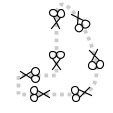
\includegraphics{turtle4.eps}
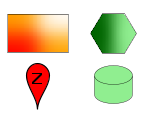
\includegraphics{turtle5.eps}
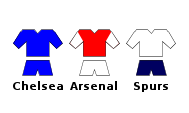
\includegraphics{turtle6.eps}
%ENDHTML
\caption{Shapes, Symbols And Patterns}
\label{turtle}
\end{figure}

%BEGINHTML
\item

Reading and displaying of geographic information
systems (GIS) datasets, text files, or tables held in a relational database
(including spatially extended databases such as PostGIS and MySQL).

Drawing routines are applied to geographic data to produce annotated and
symbolized maps and graphs.  Attributes of the geographic data control
the color, size, annotation and other characteristics of the
appearance of the geographic data.
Scalebars, legends, coordinate grids and north arrows are also available.

%ENDHTML
See Figures \ref{mapview1}, \ref{mapview3}, \ref{mapview2} and
\ref{mapview4}.

\begin{figure}
%BEGINHTML
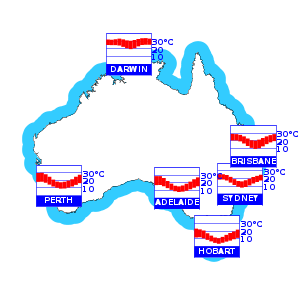
\includegraphics{mapview1.eps}
%ENDHTML
\caption[Average Monthly Temperatures]{Average Monthly Temperatures of Australian Cities (degrees Celsius)}
\label{mapview1}
\end{figure}

\begin{figure}
%BEGINHTML
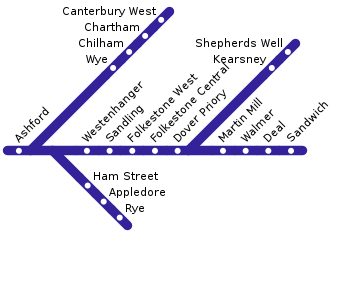
\includegraphics{mapview3.eps}
%ENDHTML
\caption{Strip Map of Railways Lines in East Kent}
\label{mapview3}
\end{figure}

\begin{figure}
%BEGINHTML

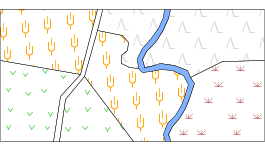
\includegraphics{mapview2.eps}
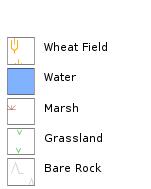
\includegraphics{mapview2legend.eps}
%ENDHTML
\vspace{1pt}
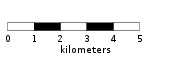
\includegraphics{mapview2scalebar.eps}
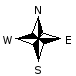
\includegraphics{mapview2north.eps}
\caption{Vegetation Classes}
\label{mapview2}
\end{figure}

\begin{figure}
%BEGINHTML
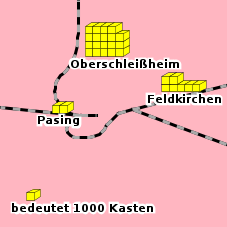
\includegraphics{mapview4.eps}
%ENDHTML
\caption{Inventory Levels at Warehouses}
\label{mapview4}
\end{figure}

%BEGINHTML

\item
Integration with the freely-available
\textit{Java Topology Suite} from Vivid Solutions
(\texttt{http://www.vividsolutions.com}).
This library provides geometric algorithms
such as buffering, point-in-polygon test and polygon intersection.

Integration with the
\textit{ogrinfo} program, part of the
freely-available OGR library
(available from \texttt{http://openev.sourceforge.net}).
This program provides access to many GIS data formats.

\item
Flexibility.  Running in one of two ways.

\begin{enumerate}
\item
As a stand-alone program for integration into
scripts and batch tasks (suitable for generating a one-off
map or a series of similar maps from a template
showing different areas, or using different criteria for each map).

\item
As a self-contained web server providing map and
graph images to a web-based application.
This also enables Mapyrus to be integrated into larger applications
(such as PHP-based applications),
with map images fetched using HTTP requests.

\end{enumerate}

\end{enumerate}

%ENDHTML

Please note that:

\begin{itemize}

\item
Mapyrus has no graphical user interface.
Commands are read from a text file prepared by the user.
Good user interfaces are
hard to design and everyone wants something slightly different.
Build a custom HTML or Java user interface on top of Mapyrus.

\item
Mapyrus cannot display three dimensional data and has nothing to do
with 3D.

\item
Mapyrus includes a sample set of about 100 ready-to-use shapes and patterns
for maps and charts (see Figure \ref{samplesymbols}
on page \pageref{samplesymbols}).
Icons found on the
internet are another good solution for display in image files.
For PostScript output, the resolution is higher and using characters
from a font such as ZapfDingbats produces better output.

\item
Mapyrus cannot reproject coordinate values in geographic data from
one projection to another.  However, this functionality
is available in spatial databases.
\end{itemize}

